% \bibliography{../src/bibliography}

This chapter introduces a neural Conditional Random Field (CRF) parser that can be used as an alternative proposal distribution for the approximate marginalization of the RNNG. The model is a span-factored CRF that independently predicts scores for labeled spans over the sentence using neural networks. The scores then interact in a tree-structured dynamic program, giving a compact description of the probability distribution over parses. This approach combines the efficient exact inference of chart-based parsing, the rich nonlinear features of neural networks, and the global training of a CRF. The chart-based approach enables efficient exact inference alowing for exact decoding and global sampling while the neural features can be complex and can condition on the entire sentence. The parser is an adaptation of the chart-based parser introduced in \citet{stern2017minimal} to global CRF training. In \citet{stern2017minimal} the model is trained with a margin-based objective, but given our interest in this model as a proposal distribution we require probabilistic training.

In this chapter:
\begin{itemize}
  \item We present the parser and describe how it is a CRF adaptation of the max-margin trained parser of \citet{stern2017minimal}.
  \item We show how several inference problems of interest can be solved exactly: parsing, entropy computation, sampling.
  \item We train the parser in a supervised fashion and show it's adequacy as a parser.
  \item We invesitage the kind of samples that are obtained from this parser, and evaluate how they affect the approximate inference in the RNNG.
\end{itemize}

\section{Model}
  The model is a CRF factored over labeled spans. Let $x$ be a sentence, and $y$ a tree from $\yieldx$. We define a function $\Psi$ that assings nonnegative scores $\Psi(\x, \y)$ and let the probability of a tree be its globally normalized score
  \begin{align}
    \label{eq:crf-model}
    p(\y \mid \x) &= \frac{\Psi(\x, \y)}{Z(\x)},
  \end{align}
  where
  \begin{align*}
    Z(\x) = \sum_{ \y \in \yieldx } \Psi(\x, \y)
  \end{align*}
  is the normalizer, or partition function, that sums over the exponential number of trees availlable for $\x$.

  To allow efficient computation of the normalizer, we let the scoring function $\Psi$ factorize over the parts of $\y$. We consider a tree as a set of labeled spans $\y_a = (A, i, j)$, thus $\y = \{ \y_a \}_{a=1}^A$, where $(A, i, j)$ indicates that $\y$ contains a label $A$ spanning the words $\langle x_{i+1}, \dots, \x_j \rangle$. The value $\Psi(\x, \y)$ is then defined as the product of the nonnegative potentials $\psi(\x, \y_a)$ as
  \begin{align}
    \Psi(\x, \y) = \prod_{a=1}^A \psi(\x, \y_a).
  \end{align}
  The function $\psi$, thus, scores each labeled span $\y_a$ seperately, but conditional on the entire sentence.

  The above model is your typical constituency parsing CRF \citep{finkel2008crf,klein2015crf}, but where those models factorize trees over \textit{anchored rules}, our model the factorizes over \textit{labeled spans},\footnote{Compare table \ref{tab:spans-rules} for the different representations of a tree.} an approach first taken in \citet{stern2017minimal}. This factorization imposes an even stronger independence assumption than that imposed by factorizatin over anchored rules. By factorizing over labeled spans, the potential function $\psi$ has no access to information about the direct substructure under the node, such as the child nodes and their split point, and the function can thus rely less on the (local) tree structure and must thus rely more on the surface features of the input sentence. It will, however, greatly reduce the size of the state-space of the dynamic programs, speeding up training and inference, and the burden of the feature function will be carried by a rich neural network parametrization. Together this will make the parser fast yet effective. This will be made clear in section \ref{sect:inference} on inference.

\section{Parametrization}
  The scoring function $\psi$ is implemented with neural networks following \citet{stern2017minimal}. Again, let $\y_a$ denote a labeled span $(A, i, j)$ in a tree $\y$, and let $\psi(\x, \y_a) > 0$ be the score of that labeled span for sentence $\x$. These local potentials can only make minimal use of structural information but they can depend on the entire sentence. This suggest the use of bidirectional RNN encodings. Let $\fw_i$ and $\bw_i$ respectively be the vectors computed by a forward and backward RNN for the word in position $i$. The representation of the span $(i, j)$ is the concatenation of the difference between the vectors on the endpoints of the span:
  \begin{align}
    \label{eq:span-feature}
    \vecs_{ij} = [\fw_j - \fw_i; \bw_i - \bw_j].
  \end{align}
  The vector $\vecs_{ij}$ represents the words $x_i^j$, and equation \ref{eq:span-feature} is illustrated in figure \ref{fig:span-feature}. The scores for each label in that position are computed from this vector using a feedforward network with output dimension $\reals^{\lvert \Lambda \rvert}$, and the score of label $A$ is given by the index corresponding to it:
  \begin{align}
    \label{eq:potential-function}
    \log \psi(\x, \y_a) = [ \ff( \vecs_{ij} ) ]_{A},
  \end{align}
  where we pretend that $A$ doubles as an index. This architecture is rightly called minimal, but it works surprisingly well: \citet{stern2017minimal} experiment with more elaborate functions based on concatenation of vectors (a strict superset of the minus approach) and biaffine scoring (inspired by \citet{dozat2016deep}), but these function improve marginally, if they do at all.

  \begin{figure}
    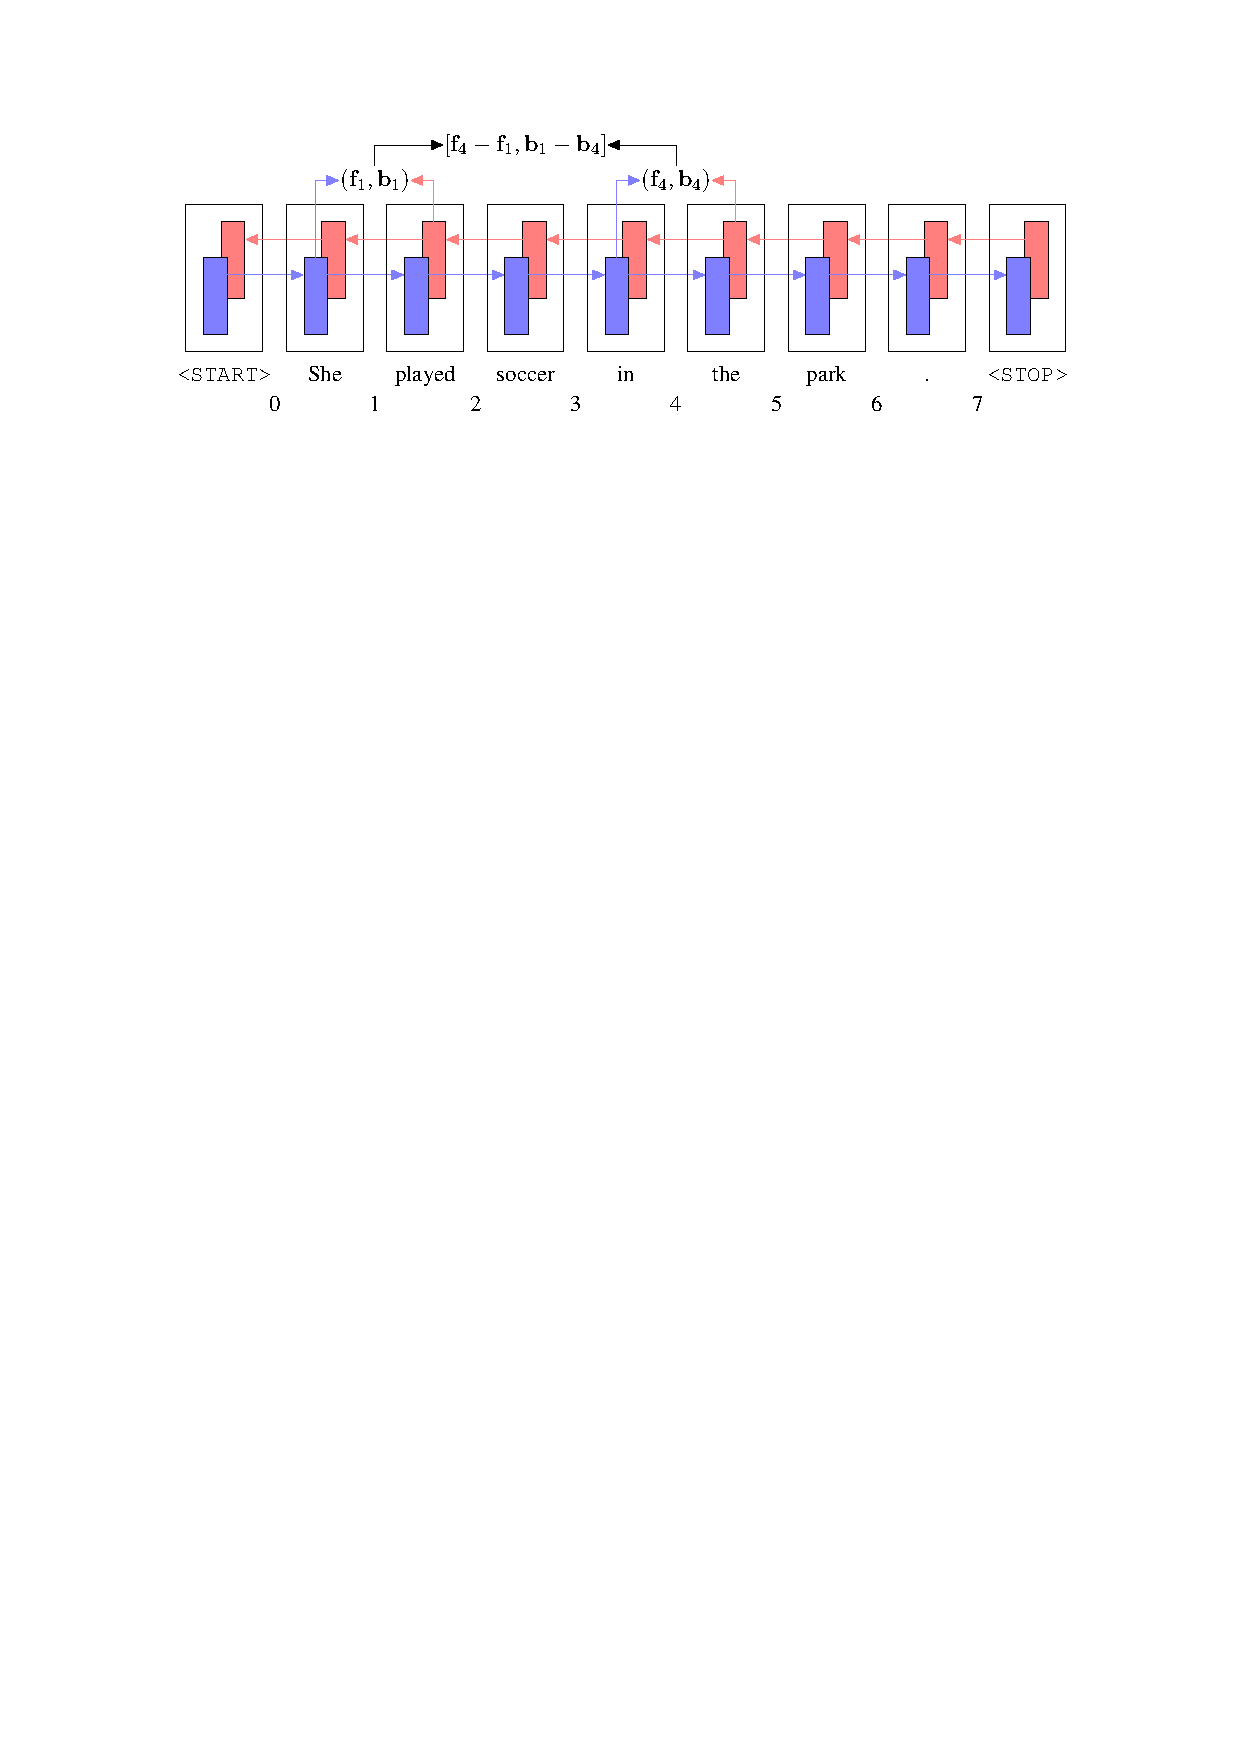
\includegraphics[width=\textwidth]{span-encoding.pdf}
    \caption{Representation for the span $(1, 4)$ computed from $\rnn$ encodings. Taken from \citet{stern2018analyis}.}
    \label{fig:span-feature}
  \end{figure}

\section{Inference}
  \label{sect:inference}
  Because our model is span-factored it allows efficient inference. In this section we describe efficient solutions to four related problems:
  \begin{itemize}
    \item Compute the normalizer $Z(\x) = \sum_{ \y \in \yieldx } \prod_{ a=1 }^{ A } \psi( \x, \y_a )$.
    \item Find the best parse $\hat{ \y } = \arg \max_{\y } p(\y  \mid \x)$
    \item Sample a tree $Y \sim P(Y \mid X = x)$. %(\cdot \mid \x)$.
    \item Compute the entropy $H(Y \mid X = x)$ over parses for $\x$.
  \end{itemize}
  These problems can be solved by instances of the \textit{inside algorithm} and \textit{outside algorithm} \citep{baker1979trainable} with differentent semirings, an insight we take from semiring parsing \citep{goodman1999semiring}. In the following derivations we will make use of the notion of a \textit{weighted hypergraph} as a compact representation of all parses and their scores \citep{gallo1993directed,klein2004parsing}, and use some of the ideas and notation of \textit{semiring parsing} \citep{goodman1999semiring,eisner2009semirings}. First we describe the structure of the parse forest specified by our CRF parser, and then derrive the particular form of the inside and outside recursions for this hypergraph from the general formulations. We refer the reader to appendix \ref{A3-crf} for background on these ideas, and the introduction of the notation.

\subsection{Weighted parse forest}
  The hypergraph $G = (\mathcal{V}, \mathcal{E})$ specified by the CRF parser has the following structure.

  The set $\mathcal{V}$ is defined relative to the sentence $\x$, and contains the invidual words of a sentence $\x$, together with all possible labeled spans over that sentence:
  \begin{align*}
    \mathcal{V} = \Big\{ \x_i \; \Big\vert \; 1 \leq i \leq n \Big\} \cup \Big\{ (A, i, j) \; \Big\vert \; A \in \Lambda, 0 \leq i < j \leq n \Big\} \cup \Big\{ (S^{\dagger}, 0, n) \Big\},
  \end{align*}
  where $(S^{\dagger}, 0, n)$ is a designated root node. The dependence on $x$ can be made explicit by writing $\mathcal{V}(x)$.

  The set of hyperedges $\mathcal{E} \subseteq 2^{\mathcal{V}} \times \mathcal{V}$ specifies all the ways that adjacent constituents can be combined to form a larger constituent, under a particular grammar. Because we (implicitly) assume a normal form grammar that contains \textit{all} possible productions, the set of hyperedges is particularly regular: the set $\mathcal{E}$ contains all edges that connect nodes $(B, i, k)$ and $(C, k, j)$ at the tail with $(A, i, j)$ at the head for all $0 \leq i < k < j \leq n$, all edges that connect $\x_i$ to $(A, i, i+1)$, and all nodes can function as top nodes:
  \begin{align*}
    \mathcal{E}
      &= \Bigg\{ \Big\langle \Big\{ (B, i, k), (C, k, j) \Big\},  (A, i, j) \Big\rangle \; \Bigg\vert \; A, B, C \in \Lambda, \; 0 \leq i < k < j \leq n \Bigg\}  \\
      &\quad\cup \Bigg\{ \Big\langle \{ \x_i \}, (A, i-1, i) \Big\rangle \; \Bigg\vert \; A \in \Lambda, \; 1 \leq i \leq n \Bigg\}  \\
      &\quad\cup \Bigg\{ \Big\langle \{ (A, 0, n) \}, (S^{\dagger}, 0, n) \Big\rangle \; \Bigg\vert \; A \in \Lambda \Bigg\}
  \end{align*}
  The three kind of edges that make up $\mathcal{E}$ are illustrated in figure \ref{fig:crf-edges}. A tree is a set of nodes $y \subseteq \mathcal{V}(x)$, and the parse forest a set of trees $\yieldx \subseteq 2^{\mathcal{V}(x)}$.

  \begin{figure}[h]
    \center
    \begin{tikzpicture}[scale=.6]
      % \documentclass[11pt]{article}
% \usepackage{tikz}
% \usepackage{amsmath,amssymb,amsfonts}
%
% \usetikzlibrary{arrows,calc}
%
% \begin{document}

% \tikzstyle{every node}=[circle, draw, inner sep=0pt, minimum size=7mm]
%
% \tikzstyle{every node}=[circle, draw, inner sep=0pt, minimum size=11mm, node distance =1 cm and 1cm ]

% \begin{tikzpicture}

\node(a){$x_i$} ;
\node(b) at ($(a)+(4.5,0)$){$B_{i}^{k}$} ;
\node(c) at ($(b)+(3,0)$){$C_{k}^{j}$} ;
\node(d) at ($(c)+(4.5,0)$){$A_{0}^{n}$} ;

\node(A1) at ($(a)+(0,3)$){$A_{i-1}^{i}$} ;
\node(A2) at ($(b)+(1.5,3)$){$A_{i}^{j}$} ;
\node(S) at ($(d)+(0,3)$){$S^{\dagger n}_{0}$} ;

\draw[->] (a) to [in=-90,out=90](A1);

\draw[->] (b) to [in=-90,out=90](A2);
\draw[->] (c) to [in=-90,out=90](A2);

\draw[->] (d) to [in=-90,out=90](S);

% \end{tikzpicture}
%
% \end{document}

    \end{tikzpicture}
    \caption{The edge-types making up the hypergraph.}
    \label{fig:crf-edges}
  \end{figure}

  We connect a semiring $\mathcal{K}$ to the hypergraph by defining the weight function as $\omega: \mathcal{E} \to \mathbb{K}$, and by accumulating the weights with its binary operations. The function $\omega$ that assigns weights to the edges is given by either the function $\psi$ or $(\log \circ \, \psi)$, depending on the semiring used. Because of this association, the function $\omega$ has a very particular property: the function effectively depends only on the \textit{head} of the edge. Given edges $e = \langle \{ u, w \}, v \rangle$ and $e' =  \langle \{ u', w' \}, v \rangle$ for $u \neq u'$ and $w \neq w'$, their weights are equal: $\omega(e) = \omega(e')$. For this reason we write $\omega(v)$ instead.\footnote{Thus implicitly defining $\omega: \mathcal{V} \to \mathbb{K}$.} This fact will allow us to greatly simplify the recursions that follow. Additionally, this means that instead of computing independent scores for each of the $O(n^3 \vert\Lambda\rvert^3)$ edges, we only need to compute scores for the $O(n^2 \vert\Lambda\rvert)$ vertices. For a scoring function like a neural network, for which computation can be relatively expensive, this will make a significant difference.

 With this structure in place, we are ready to derive the form of the inference algorithm particular to this structure.

\subsection{Inside recursion}
  The inside recursion computes quantities $\alpha(A,i,j)$ for all labels $A \in \Lambda$ and all spans $0 \leq i < j \leq n$. The quantity computed depends on the semiring used. In this section we derive the inside recursion specific to our hypergraph from the general result given.

  Let $\mathcal{K}$ be some semiring with binary operations $\oplus$ and $\otimes$ and identity elements $\bar{0}$ and $\bar{1}$. The inside recursion is given by the formula \citep{goodman1999semiring}
  \begin{align*}
    \alpha(v) =
      \begin{cases}
        \bar{1}  &  \mbox{if } I(v) = \varnothing,  \\
        \displaystyle\bigoplus_{e \in I(v)} \omega(e) \otimes \displaystyle\bigotimes_{u \in T(e)} \alpha(u)  & \mbox{otherwise.}
      \end{cases}
  \end{align*}
  Here $I(v) \subseteq E$ is the set of edges incoming at node $v$, and $T(e) \subseteq V$ is the set of nodes in the tail of edge $e$.

  At a node $v = (A, i, i+1)$ that spans one word $x_i$, the inside value is just the weight of the single edge incoming from that word:
  \begin{align}
      \label{eq:inside-base}
      \alpha(A, i, i+1) = \omega(A, i, i+1) \otimes \alpha(x_i) = \omega(A, i, i+1),
  \end{align}
  for $A \in \Lambda$, for all $0 \leq i < n$. We used the fact that $\alpha(x_i) = \bar{1}$, which follows from the fact that there are no arrows incoming at $\x_i$.

  For a general node $\alpha(A, i, j)$, $j > i + 1$, we observe that all the incoming edges have at the tail the nodes $(B, i, k)$ and $(C, k, j)$, for all $B, C \in \Lambda$ and $i < k < j$. The sum over edges thus reduces to independent sums over $B$, $C$, and $k$, and the product over the inside values at the tail reduces to the product of values $\alpha(B, i, k)$ and $\alpha(C, k, j)$. The form of $\omega$ allows us to rewrite this greatly as
  \begin{align}
    \label{eq:inside}
    \alpha(A, i, j)
      &= \bigoplus_{B \in \Lambda} \bigoplus_{C \in \Lambda} \bigoplus_{k=i+1}^{j-1} \omega(A, i, j) \otimes \alpha(B,i,k) \otimes \alpha(C,k,j) \nonumber \\
      &= \omega(A, i, j) \otimes \bigoplus_{k=i+1}^{j-1} \bigoplus_{B \in \Lambda} \alpha(B,i,k) \otimes \bigoplus_{C \in \Lambda} \alpha(C,k,j) \nonumber \\
      &= \omega(A, i, j) \otimes \bigoplus_{k=i+1}^{j-1} \sigma(i,k) \otimes \sigma(k,j),
  \end{align}
  where we've introduced the notational abbreviation
  \begin{align*}
      \sigma(i,j) &= \bigoplus_{A \in \Lambda} \alpha(A,i,j).
  \end{align*}
  Looking at \ref{eq:inside} we can see the marginalized values $\sigma(i, j)$ are all that are needed for the recursion. This suggest simplifying the recursion even further as
  \begin{align}
    \label{eq:inside-simplified}
    \sigma(i, j)
      &= \bigoplus_{A \in \Lambda} \alpha(A,i,j) \nonumber \\
      &= \Bigg[ \bigoplus_{A \in \Lambda} \omega(A, i, j) \Bigg] \otimes \Bigg[\bigoplus_{k=i+1}^{j-1} \sigma(i,k) \otimes  \sigma(k,j) \Bigg],
  \end{align}
  where we put explicit brackets to emphasize that independence of the subproblems of labeling and splitting.

\subsection{Outside recursion}
  The outside algorithm computes the quantities $\beta(A,i,j)$ for all labels $A \in \Lambda$ and all spans $0 \leq i < j \leq n$. The general recursion is given by:
  \begin{align*}
    \beta(v) =
      \begin{cases}
        \bar{1}  & \mbox{if } O(v) = \varnothing, \\
        \displaystyle\bigoplus_{e \in O(v)} \omega(w) \otimes \beta(H(e)) \otimes \displaystyle\bigotimes_{ \substack{ w \in T(e) \\ w \neq u } } \alpha(w)  & \mbox{otherwise.}
      \end{cases}
  \end{align*}
  Here, $O(v) \subseteq E$ is the set of edges outgoing from $v$, $\ie$ the edges for which $v$ is in the tail, and define $H(e) \in V$ as the node at the head of edge $e$.

  The only node without outgoing edges is the root node, and thus
  \begin{align*}
    \beta(S^{\dagger}, 0, n) = \bar{1}.
  \end{align*}
  To compute $\beta(A, i, j)$ in the general case we need to sum over all outgoing edges. These come in two kinds: either $(A, i, j)$ combines with $(C, k, i)$ to form constituent $(B, k, j)$; or either $(A, i, j)$ combines with $(C, j, k)$ to form constituent $(B, i, k)$. This corresponds to the following expression, that we can simplify by making use of the properties of $\omega$:
  \begin{align*}
    \beta(A, i, j)
      &= \bigoplus_{B \in \Lambda} \bigoplus_{C \in \Lambda} \bigoplus_{k=1}^{i-1} \omega(B, k, j) \otimes \alpha(C, k, i) \otimes \beta(B, k, j) \\
        &\qquad \oplus \bigoplus_{B \in \Lambda} \bigoplus_{C \in \Lambda} \bigoplus_{k=j+1}^{n} \omega(B, i, k) \otimes \beta(B, i, k) \otimes \alpha(C, j, k) \\
      &=  \bigoplus_{k=1}^{i-1}  \Bigg[ \bigoplus_{B \in \Lambda} \omega(B, k, j)  \otimes \beta(B, k, j) \Bigg] \otimes \Bigg[ \bigoplus_{C \in \Lambda} \alpha(C, k, i) \Bigg] \\
        &\qquad \oplus \bigoplus_{k=j+1}^{n}  \Bigg[ \bigoplus_{B \in \Lambda}  \omega(B, i, k) \otimes \beta(B, i, k) \Bigg] \otimes  \Bigg[  \bigoplus_{C \in \Lambda} \alpha(C, j, k) \Bigg] \\
      &=  \bigoplus_{k=1}^{i-1}  \sigma'(k, j) \otimes \sigma(k, i) \oplus \bigoplus_{k=j+1}^{n} \sigma'(i, k) \otimes  \sigma(j, k) \\
  \end{align*}
  where
  \begin{align*}
      \sigma(i, j) &= \bigoplus_{A \in \Lambda} \alpha(A, i, j),  \\
      \sigma'(i, j) &= \bigoplus_{A \in \Lambda} \omega(A, i, j) \beta(A, i, j).
  \end{align*}

\subsection{Solutions}
  Equiped with the two recursions and a handful of semirings we can provide the solutions promised at the outset of this section.

  \paragraph{Normalizer}
    When we intantiate the inside recursion with the real semiring, the value of $\alpha$ at the root is the normalizer:
    \begin{align*}
      \alpha(\text{S}^{\dagger}, 0, n) = Z(\x),
    \end{align*}
    and when we instantiate the inside recursion with the log-real semiring we obtain the log-normalizer
    \begin{align*}
      \alpha(\text{S}^{\dagger}, 0, n) = \log Z(\x).
    \end{align*}

  \paragraph{Parse}
    To find the viterbi tree $\hat{ \y } = \arg \max_{ \y } p(\y  \mid \x)$ and its probability $p(\hat{\y} \mid \x)$ we use the Viterbi semirings ($\cf$ examples \ref{ex:vit-weight} and \ref{ex:vit-derivation} in appendix \ref{A3-crf}). We take equation \ref{eq:inside-simplified} and use the Viterbi semiring operations to derive that the value of the best subtree spanning words $i$ to $j$ is given by
    \begin{align}
      \label{eq:viterbi-score}
      \sigma(i,j)
        &= \max_{A} [ \log \psi(A, i, j) ] + \max_{k} [\sigma(i,k) + \sigma(k,j)].
    \end{align}
    The value $\log \Psi(\x, \hat{\y})$ is then given by $\sigma(0, n)$, and  can be normalized with to give the probability
    \begin{align}
      p(\hat{y} \mid x) = \sigma(0, n) - \log Z(x).
    \end{align}
    The best label and splitpoint $\hat{A}$ and $\hat{k}$ for the span $(i, j)$ are obtained by using the argmax:
    \begin{align}
      \label{eq:viterbi-tree}
      \hat{A} &= \argmax_{ A  } \log \psi(A, i, j)  \\
      \hat{k} &= \argmax_{ k } \sigma(i, k) + \sigma(k, j),
    \end{align}
    and the best tree $\hat{y}$ is found by following back from the root down to the leaves the best splits and labels.

  \paragraph{Sample}
    Samples can be obtained by recursively sampling edges, starting at the root node $(S^{\dagger}, 0, n)$. The probability of an edges is proportional to the weight under that edge: this is precicely the inside value $\alpha$ computed in the real-semiring. An edge $e = \langle \{ u, w \}, v \rangle$, with $u = (B, i, k)$, $w = (C, k, j)$ and $v = (A, i, j)$, has probability
    \begin{align}
      \label{eq:sample}
      P(E = e)
        &= \frac{\omega(e) \otimes \bigotimes_{u \in T(e)} \alpha(u)}{\alpha(v)}  \nonumber  \\
        &= \frac{\psi(A, i, j) \, \alpha(B, i, k) \, \alpha(C, k, j)}{\alpha(A, i, j)}.
    \end{align}
    We repeat the sampling at the nodes that are in the tail of the sampled edge, until we reached the nodes that span individual words.

  \paragraph{Entropy}
    % To compute the entropy $H(Y \mid X = x)$ we need to first introduce the notion of the \textit{maginal probablity} of a node. The marginal of a node $v = (A, i, j)$ in a hypergraph is the probability that it occurs in a tree $\y$ for the sentence $\x$ as governed by the distribution $p$ that we defined on it. Let $V$ be a random variable with the hypergraph nodes $\mathcal{V}(x)$ as sample space, and define
    % \begin{align}
    %   P(V = v \mid X = \x)
    %     &\defeq \expect_Y[ \indicator_{ \{ v \in Y \} } ]  \nonumber \\
    %     &= \sum_{ \y \in \yieldx } p(\y \mid \x) \indicator_{ \{ v \in y \} }.
    % \end{align}
    %
    % The marginals can be computed from the inside and outside values computed in the real semiring as
    % \begin{align}
    %   P(V = v \mid X = \x) = \frac{\alpha(A, i, j) \, \beta(A, i, j)}{Z(\x)},
    % \end{align}
    % a result from \citep{goodman1999semiring}.\footnote{This can also be seen by noting that the product of $\alpha(A, i, j)$ and $\beta(A, i, j)$ is the sum over all trees that contain the node $v$, and $Z(\x)$ the sum over all trees in general.} The entropy can then be written as an expectation with respect to these marginals:
    % \begin{align}
    %   H(Y \mid X = x)
    %     &= - \sum_{ \y \in \yieldx } p(\y \mid \x) \log p(\y \mid \x)  \nonumber \\
    %     &= \log Z(\x) - \sum_{ \y \in \yieldx } p(\y \mid \x) \sum_{v \in \y} \log \psi(\x, v)  \nonumber \\
    %     &= \log Z(\x) - \sum_{ \y \in \yieldx } p(\y \mid \x) \sum_{ v \in \mathcal{V}(x) } \indicator_{ \{ v \in y \} } \log \psi(\x, v)  \nonumber \\
    %     &= \log Z(\x) - \sum_{ v \in \mathcal{V}(x) } \log \psi(\x, v)  \sum_{ \y \in \yieldx } \indicator_{ \{ v \in y \} } p(\y \mid \x)  \nonumber \\
    %     &= \log Z(\x) - \sum_{ v \in \mathcal{V}(x) } \log \psi(\x, v)  P(V = v \mid X = \x)  \nonumber \\
    %     &=  \log Z(\x) - \expect_V [ \log \psi(\x, V) ].
    % \end{align}
    To compute the entropy $H(Y \mid X = x)$ we need to first introduce the notion of a \textit{node maginal}. The marginal of a node $v = (A, i, j)$ in a hypergraph is the probability that it occurs in a tree $\y$ for the sentence $\x$, according to the probability distribution $p$ over trees. The node marginal $\mu(v)$ is defined as the expectation
    \begin{align}
      \label{eq:node-marginal}
      \mu(v)
        &\defeq \expect_Y[ \indicator_{ \{ v \in Y \} } ]  \nonumber \\
        &= \sum_{ \y \in \yieldx } p(\y \mid \x) \indicator_{ \{ v \in y \} }.
    \end{align}
    This can be computed from the inside and outside values computed in the real semiring as
    \begin{align}
      \mu(v) = \frac{\alpha(A, i, j) \, \beta(A, i, j)}{Z(\x)},
    \end{align}
    a result from \citep{goodman1999semiring}. This can also be seen by noting that the product of $\alpha(A, i, j)$ and $\beta(A, i, j)$ is the sum over all trees that contain the node $v$, and $Z(\x)$ the sum over all trees in general.

    The entropy, then can then be written in terms of these marginals:
    \begin{align}
      H(Y \mid X = x)
        &= - \sum_{ \y \in \yieldx } p(\y \mid \x) \log p(\y \mid \x)  \nonumber \\
        &= \log Z(\x) - \sum_{ \y \in \yieldx } p(\y \mid \x) \sum_{v \in \y} \log \psi(\x, v)  \nonumber \\
        &= \log Z(\x) - \sum_{ \y \in \yieldx } p(\y \mid \x) \sum_{ v \in \mathcal{V}(x) } \indicator_{ \{ v \in y \} } \log \psi(\x, v)  \nonumber \\
        &= \log Z(\x) - \sum_{ v \in \mathcal{V}(x) } \log \psi(\x, v)  \sum_{ \y \in \yieldx } \indicator_{ \{ v \in y \} } p(\y \mid \x)  \nonumber \\
        &= \log Z(\x) - \sum_{ v \in \mathcal{V}(x) } \log \psi(\x, v) \mu(v)
    \end{align}

\section{Traning}
The training objective is to maximize the likelihood of the training data
\begin{align*}
  \mathcal{L}(\theta)
    &= \sum_{(\x, \y) \in \dataset} \log \ptheta(\y \mid \x)
\end{align*}
with respect to the model parameters $\theta$. Writing out the objective for a single example as
\begin{align*}
  \log \ptheta(\y \mid \x) = \log \Psi(\x, \y) - \log Z(x)
\end{align*}
reveals that the maximization of this value decomposes as two separate optimizationproblems: to maximize the log-score of the example tree $\log \Psi(\x, \y)$, whilst minimizing the total weight of the parse forest $\log Z(x)$. The solution is thus to move probability mass onto the gold tree, and move mass away from \textit{all} other trees. Because the log-score of the tree decomposes as a sum of log-scores of the nodes that comprise it, the objective is effectively to \textit{increase} the scores of the labeled spans that make up the gold tree, and \textit{decrease} the scores of all other labeled spans not observed. Another effect of the factorization over parts is that this increases not only the probability of the gold tree, but the probability of all trees that share substantial substructure. It is in this precise sense that we mean that the model learns about all substructures.

We rely on automatic differentiation to compute the derivatives, but note that in principle it is possible to efficiently combine the computation of the inside and outside values with their derivatives, a fact demonstrated in \citep{eisner2009semirings} and \citep{eisner2016backprop}, and implemented in \citep{kim2017structured}. Instead, for convenience and simplicity compute the quantity $Z(x)$ and let automatic differentation do the rest.

It is fruitful to see how our global objective differs from the margin-based objective in \citep{stern2017minimal}. The margin-based objective is to maximize the difference, or `margin', between the score of the gold tree and the highest scoring, incorrect tree. Given an example pair $(\x, \y)$, the model computes the predicted tree $\hat{y}$. If the predicted tree equals the example tree, $\hat{y} = \y$, then no changes to the model are made. Otherwise, the model is updated to maximize the difference between their scores
\begin{align*}
  \Psi(\x, \y) - \Psi(\x, \hat{\y}),
\end{align*}
maximizing the score of the correct tree, and minimizing the score of the predicted tree.\footnote{The objective reported in the paper is minimizing the hinge loss $\max \Big(0, 1 - \Psi(\x, \y) + \Psi(\x, \hat{\y}) \Big)$, but the above is what is actually implementated in their code.} This objective shows a striking similarity with our CRF objective, with one very particular difference. The goal is still to maximize the score of the gold tree. But the minimization that in the CRF objective concerns all possible trees through $Z(x)$, in this objective concerns just the single tree $\hat{\y}$ that was incorrectly predicted. The scores of all other nodes not observed in either tree remain unchanched.

\section{Experiments}
  We perform three types of experiments with the CRF parser:
  \begin{itemize}
    \item We show that the model is a good supervised parser. We train the model supervised on the PTB and show the f-score on the PTB test set.
    \item We evaluate the joint RNNG with samples from the CRF parser. We compare the perplexity and fscore with RNNG case.
    \item We evauluate `how good the model is' as a sampler.
  \end{itemize}

\subsection{Supervised model}
  We investigate the following.
  \begin{itemize}
    \item We have some optimization and hyperparameter choices here. The original paper uses Adam with 0.001 and a LSTM of dimension 250, which gives the model around 2.5 million parameters. For the discriminative RRNG we use SGD with 0.1, and hidden sizes of 128 gives the model around 800,000 parameters.
    \item I suggest two experiments: (1) use the default setting from \citep{stern2017minimal} and (2) use the settings for the RNNG with a hidden size to match the 800,000 parameters.
  \end{itemize}

\subsection{Proposal model}
  We investigate the following:
  \begin{itemize}
    \item We evaluate validation F-score and perplexity.
    \item We evaluate F-score with 100 samples (as many proposal trees as possible).
    \item We evaluate perplexity with varying number of samples: 1 (argmax), 10, 20, 50, 100 (default). The peplexity evaluation with the argmax prediction gives an impression of the uncertaty in the model \citep{buys2018exact}.
    \item  We perform learning rate decay and model selection based on a development score computed with the samples from the discriminative RNNG. Undecided: should we train a separate joint RNNG with CRF samples?
  \end{itemize}

\subsection{Sampler}
  We investigate the following:
  \begin{itemize}
    \item We assess the conditional entropy of the model. This is most quantitative. Recall that conditional entropy is defined as
    \begin{equation}
      \text{H}(Y \mid X ) = \sum_{x \in \mathcal{X}} p(x)\text{H}(Y|X = x),
    \end{equation}
    where
    \begin{equation}
      \text{H}(Y|X = x) = - \sum_{y \in \mathcal{Y}} p(y|x) \log p(y|x).
    \end{equation}
    The quantity $\text{H}(Y|X = x)$ can computed exactly with the CRF parser. We estimate the quantity $\text{H}(Y|X)$ by a sum over the development dataset.
    \item We assess for some cherry picked sentences. This is more qualitative. These sentences should be difficult or ambiguous. Or they can be ungramatical when taken from the syneval dataset. We can evaluate their entropy, and the diversity of samples, for example to see if there are clear modes. We can make violinplots of the probabilities of the samples. We can compute the f-scores of the samples compared with the argmax tree.
  \end{itemize}

\section{Related work}
  The model that we presented regards a constituency tree as a collection of \textit{labeled spans} over a sentence. Earlier CRF models for constituency parsing, both log-linear and neural, factorize trees over \textit{anchored rules} \citep{finkel2008crf,klein2015crf}. This puts most of the expressiveness of the model in the state space of the dynamic program, modelling interactions between subparts of the trees through their interaction in the rules, instead of at the feature level. The model in \citet{stern2017minimal} removes part of this structure, and puts more expressiveness in the input space by using rich neural feature representations conditioning on the entire sentence. The discrete interaction between the local scores remains only at level of labeled spans. This dramatically improves the speed of this model, which will become evident in the next section.

  In recent decades, discriminative chart-parsing has moved from grammar to features: the work of \citet{hall2014less} showed how the log-linear CRF model of \cite{finkel2008crf} can work with bare unnanotated grammars when relying more heavily on surface features of the sentence, and \citet{klein2015crf} showed that the linear scoring function can be replaced with a neural network one. The work of \citep{stern2017minimal} moves one step further: the grammar is dispensed with altogether, making the model span-factored, and the scoring function is given the full power of neural networks.

  Contrast this with generative parsing based on treebank grammars, where features are not available because the models are not conditional. Instead, these models rely entirely on detailed rule information: basic treebank grammars do not parse well because the rules provide too little context, and good results can only be obtained by enriching grammars. The independence assumptions in the grammar are thus typically weakened, not strengtehened. Such approaches lexicalize rules \citep{collins2003head}, annotate the rule with parent and sibling labels \citep{klein2003accurate}, or automatically learn refinements of nonterminal categories \citep{petrov2006learning}.

  In terms of the probabilistic model, the closest predecessor to our model is the neural CRF parser of \citet{klein2015crf}, which predicts local potential for anchored rules using a feedfoward network. It differs from our approach in two ways. Their method requires a grammar, extracted from a treebank beforehand, whereas our approach implictly assumes all rules are possible rules in the grammar. Secondly, their scoring function conditions only on the parts of the sentence directly under the rule, dictated by the use of a feedforward network, whereas our scoring function computes a score bassed on representations computed from the entire sequence.

  % Earlier work on CRF parsing consider a tree as a collection of anchored rule productions productions \cite{finkel2008crf,klein2015crf}, and hence define the score of a tree as the product over clique potentials on anchored rules:
  % \begin{align}
  %   \log\psi(A \to B \;C, i, k, j) = \log\psi(A, i, j)\\
  % \end{align}
  % discarding the rest of the span information. The function is then defined as
  % \begin{align}
  %   \label{eq:span-score}
  %   \log\psi(A, i, j) &\defeq s(i, j, A),
  % \end{align}
  % Note that the potential function as defined in \ref{eq:rule-score} disregards most of the information in a binary rule. In particular we see that $B$, $C$ and $k$, the labels and split-point of the children, are discarded.

  % \section{Related work}
  %   Here I describe related work, and in particular earlier approaches to (neural) CRF-parsing.
  %   \begin{enumerate}
  %     \item Of course \citep{stern2017minimal}
  %     \item CRFs \citep{sutton2012crf}
  %     \item CRF parsing with linear and nonlinear features \citep{finkel2008crf,klein2015crf}
  %     \item Attempts to simplify the grammar and thus the state-space of the dynamic program \citep{hall2014less}.
  %     \item Recent extension of \citet{stern2017minimal}, with same model but different features \citep{kitaev2018attentive}.
  %   \end{enumerate}
